\subsection{Introducción}
	Vaadin\cite{vaadin} es un framework de desarrollo de SPA que permite escribir el código de dichas aplicaciones en Java o en cualquier otro lenguaje soportado por la JVM 1.6+. Esto permite la programación de la interfaz gráfica en lenguajes como Java 8, Scala o Groovy, por ejemplo.


	Una de las características diferenciadores de Vaadin es que, contrario a las librerías y frameworks de JavaScript típicas, presenta una arquitectura centrada en el servidor, lo que implica que la mayoría de la lógica es ejecutada en los servidores remotos. Del lado del cliente, Vaadin está construido encima de Google Web Toolkit, con el que puede extenderse.


	En este proyecto, Vaadin se encargara de realizar la comunicación entre el cliente y el servidor. De esta forma, será capaz de enviar y recibir datos, eventos y peticiones entre el componente Javascript (cliente) y el servidor.


	\begin{figure}[!tb]
		\centering
		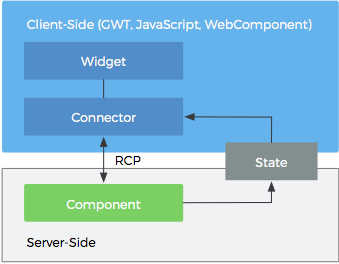
\includegraphics[scale=1.5]{schema.png}
		\caption{Esquema Cliente-Servidor}\label{fig:schema}
	\end{figure}
 			
\subsection{Ejemplo}
 	La finalidad de este ejemplo es realizar una sencilla comunicación entre un componente Javascript y un proyecto implementado en Java utilizando para ello el soporte de Vaadin. Por lo tanto se creaará un componente en Vaadin que podrá ser utilizado posteriormente en diversos proyectos.
 	
 	\begin{figure}[!tb]
 		\centering
 		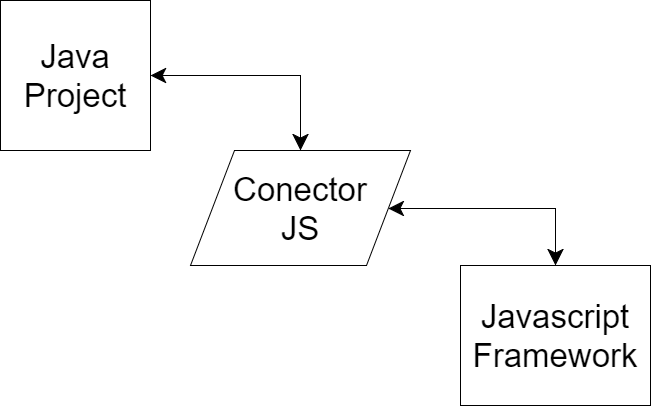
\includegraphics[scale=0.5]{vaadinInteraction.png}
 		\caption{Interacción Vaadin}\label{fig:vaadinInteraction}
 	\end{figure}
 	
 	El primer paso es diferenciar las partes que actúan en esta comunicación, para ello la Figura~\ref{fig:vaadinInteraction} representa brevemente esta interacción. Como podemos observar, se consta de tres módulos bien diferenciados. El primer módulo se corresponde con el proyecto implementado en Java. El segundo con el conector en javascript que servirá de comunicador o intermediario entre la librería Javascript y el proyecto. El último se corresponde con la librería Javascript, un ejemplo de esta es GoJS, explicada previamente, por lo tanto, no se mencionará más de ella más allá de que es la encargada del entorno gráfico.
 	
 	
 	\subsubsection{Java Project}
 			
 	En este proyecto la pieza central que será la encargada de comunicarse con el conector será un componente abstracto que implementa Vaadin para llevar a cabo esta finalidad. 
 	
 	Este componente consta de dos partes, por un lado tiene una clase que extiende de \emph{AbstractJavaScriptComponent} (Figura~\ref{fig:componenteVaadin}~,~Línea 2) que será la pieza que posea el contexto para comunicarse con el conector, además, en esta parte se especificarán todos los ficheros javascript u hojas de estilo que sean necesarios (Figura~\ref{fig:componenteVaadin}~,~Línea 1). Por otro lado el estado de dicho componente, que se encargará de asegurar la integridad de los elementos que existen dentro del componente y extenderá de \emph{JavaScriptComponentState} (Figura~\ref{fig:estadoComponenteVaadin}~,~Línea 1).
 	
 	\begin{figure}[!tb]
 		\centering
 		\begin{lstlisting}[language=Java]
	 	@JavaScript({ "connector.js" })
	 	public class Component extends AbstractJavaScriptComponent {
		 	public Component(String content) {
		 		getState().content = content;
		 	}
		 	
		 	@Override
		 	protected ComponentState getState() {
		 		return (ComponentState) super.getState();
		 	}
	 	}
 		\end{lstlisting}
 		\caption{Componente Vaadin}
 		\label{fig:componenteVaadin}
 	\end{figure}
 
 
 \begin{figure}[!tb]
 	\centering
 	\begin{lstlisting}[language=Java]
	public class ComponentState extends JavaScriptComponentState {
		public String content;
	}
 	\end{lstlisting}
 	\caption{Estado Componente Vaadin}
 	\label{fig:estadoComponenteVaadin}
 \end{figure}


	La comunicación del componente con el conector se puede realizar de varias formas, las más comunes son:
	\begin{itemize}
		\item  Cambiando el estado del componente, ya que se ejecutará automáticamente una llamada en el conector por dicho cambio.
		\item  Haciendo una llamada al conector mediante una función previamente publicada (Figura~\ref{fig:callfunction}~,~Línea 1). De esta forma se puede elegir la función a la que llamar pasando una serie de parámetros.
	\end{itemize}

\begin{figure}[!tb]
	\centering
	\begin{lstlisting}[language=JavaScript]
	callFunction("updateState",content);
	\end{lstlisting}
	\caption{Llamada al conector}
	\label{fig:callfunction}
\end{figure}
 			
 			
 			
 	\subsubsection{Javascript Connector}	
 	
 	
 	El conector es el encargado de comunicarse con ambos lados, es decir, con el proyecto Java y el framework Javascript.
 	
 	Se empieza con la declaración de la localización del conector bajo la nomenclatura \emph{window+dirección+nombre del conector}, y después se especifica el conector (Figura~\ref{fig:conectorDesc}~,~Línea 1).
 	
 	El conector se compone principalmente de una función que se ejecuta cuando el estado del Componente en Vaadin cambia (Figura~\ref{fig:conectorDesc}~,~Líneas~04-06). Además, se le pueden añadir todas las funciones necesarias para el correcto funcionamiento (Figura~\ref{fig:conectorDesc}~,~Líneas~08-10). Como se puede observar en la Figura~\ref{fig:conectorDesc}~,~Línea~03, se crea un componente, este componente se correspondería, aplicando el caso al que se utilizará posteriormente en el proyecto, a GoJS, más concretamente a la descripción que se explica en el ejemplo del mismo.
 	
 	
 	\begin{figure}[!tb]
 		\centering
 		\begin{lstlisting}[language=JavaScript]
 		window.urlPaquete_connector = function() {

 			var mycomponent = new mylibrary.MyComponent(this.getElement());
		 	
		 	this.onStateChange = function() {
		 		mycomponent.content = this.getState().content; 
		 	}
		 	
		 	this.updateState = function(content){
		 		mycomponent.content = content;
		 	}
	 	}
 		\end{lstlisting}
 		\caption{Conector}
 		\label{fig:conectorDesc}
 	\end{figure}

	En conclusión, se ha explicado un ejemplo de interacción del componente Vaadin con un Framework Javascript a través de un conector Javascript.
 	
 	
 	
 			